\chapter{Inleiding}
\label{hoofdstuk:inleiding}

\section{Fysisch gebaseerd renderen}
\paragraph{Ray tracing}
\textit{Ray tracing} is een computergrafiek techniek voor fysisch gebaseerd renderen. Het vormt een beschrijving van een 3D scene om tot een fotorealistische 2D afbeelding. Een camera wordt op een bepaalde positie in de scene geplaatst en een afbeeldingsvlak, opgedeeld in pixels, wordt ervoor geplaatst. Door elke pixel worden één (of meerdere stralen) gestuurd. Deze stralen worden zichtstralen genoemd en de kleur van hun dichtste intersectiepunt met de scene, bepaalt de kleur van de pixel. Figuur \ref{fig:raytracing} toont dit visueel.\\

\begin{figure}
    \centering
    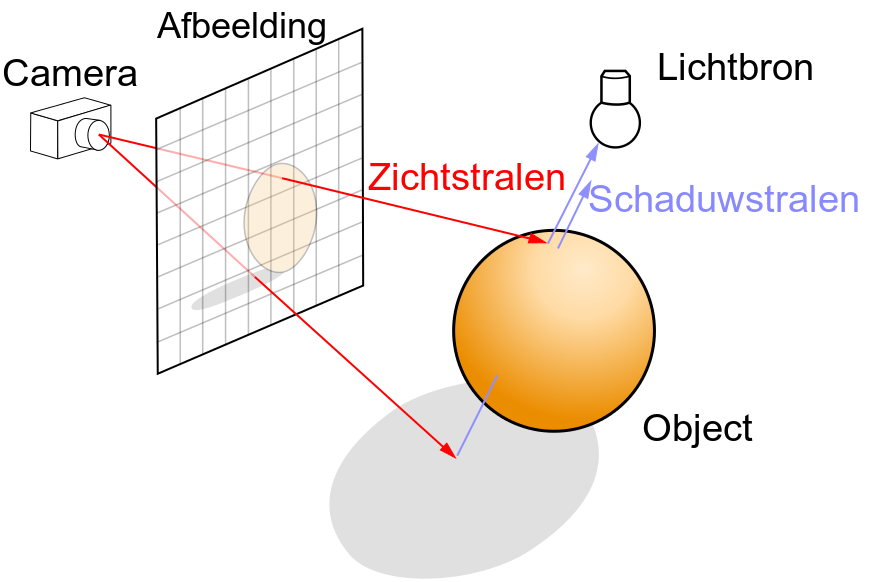
\includegraphics[width=0.5\linewidth]{img/ray-tracing}
    \caption[Visuele voorstelling van \textit{ray tracing}]%
{Visuele voorstelling van \textit{ray tracing} - \small Door elke pixel worden één of meerdere zichtstralen gestuurd. Schaduwstralen worden gebruikt om de belichting in de scene realistisch te maken. Deze afbeelding is een aangepaste versie van een afbeelding op \url{https://en.wikipedia.org/wiki/Ray_tracing_(graphics)}}
    \label{fig:raytracing}    
\end{figure}

Om realistische afbeeldingen te maken, wordt belichting in rekening gebracht. De eenvoudigste vorm van belichting is directe belichting waarbij een punt donker is als er niet rechtstreeks licht van een lichtbron op valt. Om dit te ondersteunen in \textit{ray tracing} wordt gebruikt gemaakt van schaduwstralen. Dit zijn stralen van het punt naar de lichtbron.  Deze schaduwstralen worden geïntersecteerd met de scene, als een intersectiepunt tussen het punt en de lichtbron gevonden wordt, is de lichtbron niet zichtbaar.  Bij elke intersectie wordt aan de hand van schaduwstralen gekeken of het punt belicht wordt of niet, als het niet belicht wordt, is de kleur zwart. Voor indirecte belichting is \textit{path tracing} een veelgebruikte techniek. \textit{Path tracing} reflecteert stralen in het intersectiepunt afhankelijk van het materiaal en als deze straal na een aantal botsingen een lichtbron raakt, krijgt het intersectiepunt een belichting van die lichtbron.    

%  voor realistische beeldgeneratie + referentie,


\paragraph{Acceleratiestructuren}
Het doel van acceleratiestructuren is om het aantal straal-driehoek intersecties te verminderen.
De simpelste acceleratiestructuur bestaat uit het omhullend volume van de scene.
Testen op intersectie met de driehoeken in de scene gebeurt dan enkel als dit omhullend volume intersecteert met de straal.
Deze acceleratiestructuur kan worden uitgebreid tot een boomstructuur door dit volume recursief op te delen in kindvolumes.
Binaire bomen delen elk omhullend volume op in twee nieuwe volumes, andere acceleratiestructuren zoals bijvoorbeeld octrees, delen het volume op in meer dan twee volumes.
\\

Het volume kan worden opgedeeld op twee manieren: volgens objecten of volgens ruimte.
Bij opdeling volgens objecten worden de objecten binnen het volume opgedeeld in meerdere disjuncte groepen en de kindvolumes zijn de omhullende volumes van deze groepen.
Na deze opdeling zit elk object in exact één van deze nieuwe volumes, maar de volumes kunnen overlappen.
Een voorbeeld van een acceleratiestructuur waarbij de opdeling volgens objecten gebeurt is de \textit{Bounding Volume Hierarchy} ($\symBVH$).
Opdeling volgens ruimte betekent dat de ruimte in het volume wordt opgedeeld in meerdere delen.
Na deze opdeling overlappen deze nieuwe volumes niet, maar een object ligt nu in minstens één (en mogelijks in meerdere) kindvolume(s).
De $\symBSP$ boom deelt de ruimte van het volume steeds op in twee kindvolumes.
% TODO: check if all abbrev are listed and defined at first usage

\section{Doelstelling}
In de praktijk wordt altijd een specifiek soort $\symBSP$ boom gebruikt: de $\symKd$ boom.
Deze boom splitst knopen enkel op via asgealigneerde splitsingsvlakken waardoor hij een aantal computationele voordelen heeft tijdens het bouwen en doorkruisen van de boom.
Het nadeel hiervan is dat de $\symKd$ boom zich niet goed kan aanpassen aan complexe niet-asgealigneerde geometrie waardoor bepaalde regio's veel straal-driehoekintersecties nodig hebben.\\

Algemene $\symBSP$ bomen kunnen hiervoor theoretisch gezien een oplossing bieden.
Het ontwerpen van een algemene $\symBSP$ boom die efficiënter is dan de $\symKd$ boom bij het \textit{ray tracen}, is een moeilijk probleem.
Eén van de moeilijkheden bij het bouwen van een algemene $\symBSP$ boom is het kiezen van goede splitsingsvlakken uit het grote aantal mogelijke splitsingsvlakken.
In tegenstelling tot de $\symKd$ boom, waarbij enkel asgealigneerde vlakken mogelijk zijn, zijn alle vlakken mogelijk bij een algemene $\symBSP$ boom.
In deze masterproef wordt onderzocht of het mogelijk is om goede splitsingvlakken te bepalen afhankelijk van de normalen van de driehoeken in de scene.\\

De oplossing die in deze tekst naar voorgeschoven wordt, is een nieuw soort algemene $\symBSP$ boom: de $\symBSPsweep$ boom.
De $\symBSPsweep$ boom laat toe om in elke knoop een aantal richtingen te bepalen afhankelijk van de driehoeken in die knoop
en het beste vlak van alle vlakken met als normaal één van die richtingen, wordt gebruikt om de knoop te splitsen.

\section{Structuur van de tekst}
Hoofdstuk \ref{hoofdstuk:voorgaand-werk} bespreekt de bestaande soorten $\symBSP$ bomen. Hoofdstuk \ref{hoofdstuk:bsp-sweep} start met het beschrijven van het algemene concept van de nieuwe $\symBSPsweep$ boom. Daarna worden drie varianten van dit type boom besproken, één die random richtingen gebruikt en twee die gebruik maken van de normalen. Hoofdstuk \ref{hoofdstuk:implementatie} beschrijft de implementaties, inclusief gelijkenissen en verschillen, van de verschillende bestaande en nieuwe $\symBSP$ bomen. Hoofdstuk \ref{hoofdstuk:resultaten} bespreekt de resultaten van de nieuwe $\symBSPsweep$ bomen in functie van het aantal richtingen en vergelijkt de kwaliteit van de nieuwe bomen met de bestaande $\symBSP$ bomen.

%%% Local Variables: 
%%% mode: latex
%%% TeX-master: "masterproef"
%%% End: 
